\uuid{Oz1G}
\exo7id{5815}
\auteur{rouget}
\organisation{exo7}
\datecreate{2010-10-16}
\isIndication{false}
\isCorrection{true}
\chapitre{Conique}
\sousChapitre{Conique}

\contenu{
\texte{
Etudier les courbes dont une équation en repère orthonormé est :
}
\begin{enumerate}
    \item \question{$2x^2+6xy+5y^2+4x+6y+1 = 0$.}
\reponse{Pour $(x,y)\in\Rr^2$, posons $f(x,y) =2x^2+6xy+5y^2+4x+6y+1$  et $Q((x,y)) = 2x^2+6xy+5y^2$.

 
Le discriminant de cette conique est $\Delta=2\times5 - 3^2 = 1>0$ et la courbe $(\Gamma)$ est du genre ellipse c'est-à-dire soit une ellipse, éventuellement un cercle, soit un point, soit l'ensemble vide.

\textbf{Point critique.}

\begin{center}
$\left\{
\begin{array}{l}
\rule[-5mm]{0mm}{0mm}\frac{\partial f}{\partial x}(x,y)=0\\
\frac{\partial f}{\partial y}(x,y)=0
\end{array}
\right.\Leftrightarrow
\left\{
\begin{array}{l}
4x+6y+4=0\\
6x+10y+6=0
\end{array}
\right.\Leftrightarrow x=-1\;\text{et}\;y=0$.
\end{center}

On note $\Omega$ le point de coordonnées $(-1,0)$ dans le repère $\mathcal{R}$.

\textbf{Réduction de $Q$ en base orthonormée.}
La matrice de $Q$ dans la base $(i,j)$ est $\left(
\begin{array}{cc}
2&3\\
3&5
\end{array}
\right)$. Son polynôme caractéristique est $\chi_A = X^2-7X+1$ et les valeurs propres de $A$ sont $\alpha=\frac{7+3\sqrt{5}}{2}$  et $\beta=\frac{7-3\sqrt{5}}{2}$.

$\text{Ker}(A-\alpha I_2)$ est la droite d'équation $-(1+\sqrt{5})x + 2y=0$ et est engendrée par le vecteur unitaire $e_1=\frac{1}{\sqrt{10+2\sqrt{5}}}(2,1+\sqrt{5})$. Puis $\text{Ker}(A-\alpha I_2)$ est la droite d'équation $-(1-\sqrt{5})x + 2y=0$ et est engendrée par le vecteur unitaire $e_2=\frac{1}{\sqrt{10-2\sqrt{5}}}(2,1-\sqrt{5})$.

\textbf{Equation réduite de $(\Gamma)$ dans $\mathcal{R}'=(\Omega,e_1,e_2))$.}

Les termes de degré $1$ disparaissent car $\Omega$ est l'origine de $\mathcal{R}'$ et d'autre part, $Q(xi+yj) = Q(Xe_1+Ye_2) =\alpha X^2+\beta Y^2$.

Il manque simplement la constante mais si on effectue le changement de variables $x = x_0+aX+bY$ et $y = y_0+cX+dY$, la constante est bien sûr $f((x_0,y_0))$. Donc une équation cartésienne de $(\Gamma)$ dans $\mathcal{R}'$ est $\alpha X^2+\beta Y^2+f((-1,0))= 0$ ce qui s'écrit encore

\begin{center}
$\frac{7+3\sqrt{5}}{2}X^2+\frac{7-3\sqrt{5}}{2}Y^2 = 1$.
\end{center}

\textbf{Eléménts caractéristiques de la courbe $(\Gamma)$ dans le repère $\mathcal{R}'$.}

$(\Gamma)$ est une ellipse de centre $\Omega$, d'axe focal $(\Omega Y)$ car $a=\frac{1}{\sqrt{\frac{7+3\sqrt{5}}{2}}}<\frac{1}{\sqrt{\frac{7-3\sqrt{5}}{2}}}=b$ et d'axe non focal $(\Omega X)$.

- \emph{Centre} $\Omega(0,0)_{\mathcal{R}'}$.
 
 
- \emph{Excentricité} $c^2=b^2-a^2 =\frac{2}{7-3\sqrt{5}}-\frac{2}{7+3\sqrt{5}}=3\sqrt{5}$ puis $e^2 =\left(\frac{c}{b}\right)^2=\frac{3\sqrt{5}}{7+3\sqrt{5}}=\frac{-45+21\sqrt{5}}{4}$ et 

$e=\frac{1}{2}\sqrt{-45+21\sqrt{5}}= 0,69...$
 
- \emph{Sommets} $A\left(\sqrt{\frac{7-3\sqrt{5}}{2}},0\right)_{\mathcal{R}'}$  $A'\left(-\sqrt{\frac{7-3\sqrt{5}}{2}},0\right)_{\mathcal{R}'}$  $B\left(0,\sqrt{\frac{7+3\sqrt{5}}{2}}\right)_{\mathcal{R}'}$  $B'\left(0,-\sqrt{\frac{7+3\sqrt{5}}{2}}\right)_{\mathcal{R}'}$ 

- \emph{Foyers} $\Omega F =\Omega F'=c=\sqrt{3\sqrt{5}}$  et puisque $(\Omega Y)$ est l'axe focal, $F(0,\sqrt{3\sqrt{5}})$ et $F'(0,-\sqrt{3\sqrt{5}})$. 

- \emph{Directrices} $\Omega K =\Omega K'=\frac{b}{e}=2\sqrt{\frac{2}{(7-3\sqrt{5})(-45+21\sqrt{5})}}=\frac{2}{7-3\sqrt{5}}\sqrt{\frac{2}{3\sqrt{5}}}=\frac{7+3\sqrt{5}}{\sqrt{6\sqrt{5}}}$ et donc 

$(D)$ : $Y =\frac{7+3\sqrt{5}}{\sqrt{6\sqrt{5}}}$ et $(D')$ : $Y = -\frac{7+3\sqrt{5}}{\sqrt{6\sqrt{5}}}$. 

\textbf{Eléménts caractéristiques de $(\Gamma)$ dans $\mathcal{R}$.}

Les formules de changement de repère s'écrivent $\left(\begin{array}{c}
x\\
y
\end{array}
\right)=\left(
\begin{array}{cc}
\frac{2}{\sqrt{10+2\sqrt{5}}}&\frac{2}{\sqrt{10+2\sqrt{5}}}\\
\frac{1+\sqrt{5}}{\sqrt{10+2\sqrt{5}}}&\frac{1-\sqrt{5}}{\sqrt{10-2\sqrt{5}}}
\end{array}
\right)\left(\begin{array}{c}
X\\
Y
\end{array}
\right)+\left(\begin{array}{c}
-1\\
0
\end{array}
\right)$.

- \emph{Centre} $\Omega(-1,0)_{\mathcal{R}}$ et excentricité $e =\frac{1}{2}\sqrt{-45+21\sqrt{5}}= 0,69...$

- \emph{Sommets} $A\left(
-1+\sqrt{\frac{25-11\sqrt{5}}{10}},
\sqrt{\frac{5-2\sqrt{5}}{5}}
\right)_{\mathcal{R}}$  et $A'\left(
-1-\sqrt{\frac{25-11\sqrt{5}}{10}},
-\sqrt{\frac{5-2\sqrt{5}}{5}}
\right)_{\mathcal{R}}$  puis

$B\left(
-1+\sqrt{\frac{25+11\sqrt{5}}{10}},
\sqrt{\frac{5+2\sqrt{5}}{5}}
\right)_{\mathcal{R}}$  et $B'\left(
-1-\sqrt{\frac{25+11\sqrt{5}}{10}},
\sqrt{\frac{5+2\sqrt{5}}{5}}
\right)_{\mathcal{R}}$

- \emph{Foyers} $F\left(
-1+\sqrt{\frac{3(\sqrt{5}-1)}{2}},
\sqrt{\frac{3(\sqrt{5}-1)}{2}}
\right)_{\mathcal{R}}$  et $F'\left(
-1-\sqrt{\frac{3(\sqrt{5}-1)}{2}},
-\sqrt{\frac{3(\sqrt{5}-1)}{2}}
\right)_{\mathcal{R}}$ 

-\emph{Directrices} $(D)$ :  $\frac{1}{\sqrt{10-2\sqrt{5}}}(2(x+1)+(1-\sqrt{5})y) =\frac{7+3\sqrt{5}}{\sqrt{6\sqrt{5}}}$  et 
$(D')$ :  $\frac{1}{\sqrt{10-2\sqrt{5}}}(2(x+1)+(1-\sqrt{5})y) =-\frac{7+3\sqrt{5}}{\sqrt{6\sqrt{5}}}$.

$$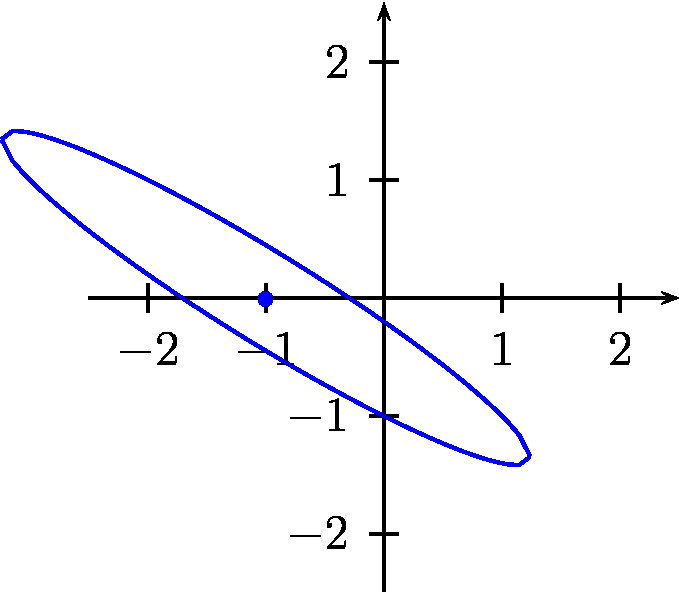
\includegraphics{../images/img005815-1}$$}
    \item \question{$x^2+2xy+y^2 +3x-2y+1 = 0$.}
\reponse{Pour $(x,y)\in\Rr^2$, posons $f(x,y) =x^2+2xy+y^2+3x-2y+1$ puis $Q((x,y)) = x^2+2xy+y^2 = (x+y)^2$. $Q$ est de rang $1$ et donc $(\Gamma)$ est du genre parabole c'est-à-dire soit une parabole, soit une réunion de deux droites parallèles éventuellement confondues, soit l'ensemble vide.

Si $(\Gamma)$ est non vide, $(\Gamma)$ est une conique est de direction asymptotique d'équation $y = - x$ (fournie par $Q(x,y)= 0$).

\textbf{1ère étude.} On étudie l'intersection de $(\Gamma)$ avec une perpendiculaire quelconque à sa direction. Soit $(D_k)$ la droite d'équation $y = x+k$, $k\in\Rr$.

L'équation aux abscisses des points d'intersection de $(\Gamma)$ et $(D_k)$ est
$x^2+2x(x+k)+(x+k)^2+3x-2(x+k)+1=0$ ou encore 

\begin{center}
$4x^2+(4k+1)x+k^2-2k+1=0$.
\end{center}

Le discriminant de cette équation est $\Delta=(4k+1)^2-16(k^2-2k+1) = 40k-15$. Puisque ce discriminant change de signe, $(\Gamma)$ est une parabole.

Le discriminant est nul pour $k=\frac{3}{8}$ ce qui founit la tangente au sommet $(T)$ : $y=x+\frac{3}{8}$ et aussi le sommet :

\begin{center}
$x_S=-\frac{4\times\frac{3}{8}+1}{2\times4}= -\frac{5}{16}$  et $y_S =x_S+\frac{3}{8}=\frac{1}{16}$.
\end{center}

Le sommet de la parabole $(\Gamma)$ est le point $S\left(-\frac{5}{16},\frac{1}{16}\right)$.

L'axe focal est la perpendiculaire à la droite $(T)$ en $S$. Une équation de l'axe focal $(\Delta)$ est $y+\frac{5}{16}=-\left(x-\frac{1}{16}\right)$ ou encore $y = -x-\frac{1}{4}$.

Pour obtenir le paramètre, le foyer et la directrice, on constate tout d'abord au vu du signe du discriminant calculé plus haut que $F = S+\frac{p}{2}\left(-\frac{1}{\sqrt{2}},\frac{1}{\sqrt{2}}\right)$    et $K= S-\frac{p}{2}\left(-\frac{1}{\sqrt{2}},\frac{1}{\sqrt{2}}\right)$.

Il ne manque plus que le paramètre $p$. Soit $M$ l'un des deux points de $(\Gamma)$ situé sur la parallèle à la tangente au sommet passant par $F$. La construction usuelle d'une parabole point par point montre que le quadrilatère $(M,F,K,H)$ est un carré. Le paramètre $p$ cherché est alors $p=FK=FM$.

 
Dans ce cas, la droite $(MK)$ est la tangente à $(\Gamma)$ en $M$ et la bissectrice de l'angle des droites $(D)$ et $(\Delta)$. Cette tangente est donc parallèle à l'un des axes de coordonnées.

L'équation générale de la tangente en un point $(x_0,y_0)$ de $(\Gamma)$ est fournie par la règle de dédoublement des termes : $xx_0+xy_0+x_0y+yy_0+\frac{3}{2}(x+ x_0)-(y+y_0)+1=0$ ou encore $x\left(x_0+y_0+\frac{3}{2}\right)+y(x_0+y_0-1)+ x_0-y_0+1=0$. Cette tangente est parallèle à l'un des axes de coordonnées si et seulement si $x_0+y_0+\frac{3}{2}=0$ ou $x_0+y_0-1=0$.

$M$ est donc sur l'une des deux droites $(\Delta_1)$ : $x+y+\frac{3}{2}=0$ ou $(\Delta_2)$ : $x+y-1=0$ qui sont toutes deux parallèles à l'axe focal $(\Delta)$ : $x+y+\frac{1}{4}=0$.

$p$ est donc aussi la distance de $(\Delta)$ à l'une quelconque de ces deux droites ou la distance d'un point quelconque de $(\Delta)$ à la droite $(\Delta_1)$. Comme le point de coordonnées $\left(-\frac{1}{4},0\right)$ est sur $(\Delta)$,

\begin{center}
$p=\frac{\left|-\frac{1}{4}+0+\frac{3}{2}\right|}{\sqrt{1^2+1^2}}=\frac{5}{4\sqrt{2}}$
\end{center}

puis $F=S+\frac{5}{8\sqrt{2}}\left(-\frac{1}{\sqrt{2}},\frac{1}{\sqrt{2}}\right)=\left(-\frac{5}{16}-\frac{5}{16},\frac{1}{16}+\frac{5}{16}\right)=\left(-\frac{5}{8},\frac{3}{8}\right)$  
et $K =S-\frac{5}{8\sqrt{2}}\left(-\frac{1}{\sqrt{2}},\frac{1}{\sqrt{2}}\right)=\left(-\frac{5}{16}+\frac{5}{16},\frac{1}{16}-\frac{5}{16}\right)=\left(0,-\frac{1}{4}\right)$ de sorte que la directrice $(D)$ a pour équation $y=x-\frac{1}{4}$.

$$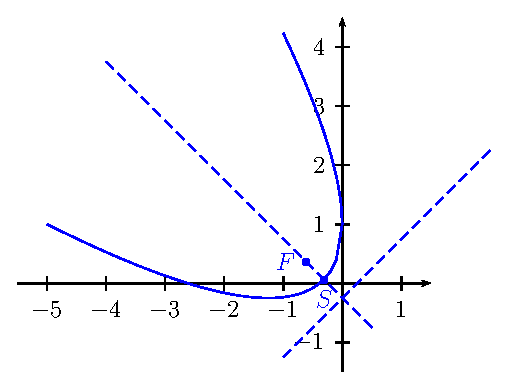
\includegraphics{../images/img005815-2}$$



\textbf{2ème étude.} On pose $X =\frac{1}{\sqrt{2}}(x+y)$ et $Y=\frac{1}{\sqrt{2}}(-x+y)$ ou encore $x=\frac{1}{\sqrt{2}}(X-Y)$ et $y=\frac{1}{\sqrt{2}}(X+Y)$ ce qui correspond au changement de bases orthonormées de matrice $P=\left(
\begin{array}{cc}
\frac{1}{\sqrt{2}}&-\frac{1}{\sqrt{2}}\\
\rule{0mm}{6mm}\frac{1}{\sqrt{2}}&\frac{1}{\sqrt{2}}
\end{array}
\right)$. On note $(e_1,e_2)$ la famille de matrice $P$ dans la base $(i,j)$. Déterminons une équation de $(\Gamma)$ dans le repère $\mathcal{R}'=(O,e_1,e_2)$.

\begin{align*}\ensuremath
(x+y)^2+3x-2y+1=0&\Leftrightarrow2X^2+\frac{3}{\sqrt{2}}(X-Y)-\frac{2}{\sqrt{2}}(X+Y)+1 = 0\Leftrightarrow2X^2+\frac{1}{\sqrt{2}}X-\frac{5}{\sqrt{2}}Y+1=0\\
 &\Leftrightarrow2\left(X+\frac{1}{4\sqrt{2}}\right)^2-\frac{1}{16}-\frac{5}{\sqrt{2}}Y+1=0\Leftrightarrow\left(X+\frac{1}{4\sqrt{2}}\right)^2=\frac{5}{2\sqrt{2}}\left(Y-\frac{3}{8\sqrt{2}}\right).
\end{align*}

\textbf{Eléments de $(\Gamma)$ dans $\mathcal{R}'$.}

- $(\Gamma)$ est une parabole de \emph{sommet} $S\left(-\frac{1}{4\sqrt{2}},\frac{3}{8\sqrt{2}}\right)_{\mathcal{R}'}$.

- \emph{Paramètre} $p =\frac{5}{4\sqrt{2}}$. L'axe focal de $(\Gamma)$ est l'axe $(SY)$ et le foyer a une ordonnée strictement supérieure à $Y_S$. 

- \emph{Foyer} $F = S+\frac{5}{8\sqrt{2}}(0,1)_{\mathcal{R}'}=\left(-\frac{1}{4\sqrt{2}},\frac{1}{\sqrt{2}}\right)_{\mathcal{R}'}$.

- \emph{Directrice} $K = S-\frac{5}{8\sqrt{2}}(0,1)_{\mathcal{R}'}=\left(-\frac{1}{4\sqrt{2}},-\frac{1}{4\sqrt{2}}\right)_{\mathcal{R}'}$ et donc $(D)$ : $Y = -\frac{1}{4\sqrt{2}}$.

 

\textbf{Eléments de la parabole $(\Gamma)$ dans le repère $\mathcal{R}$.}

- \emph{Paramètre} $p =\frac{5}{4\sqrt{2}}$. \emph{Sommet} $S=\left(\frac{1}{\sqrt{2}}X_S-\frac{1}{\sqrt{2}}Y_S,\frac{1}{\sqrt{2}}X_S+\frac{1}{\sqrt{2}}Y_S\right)_{\mathcal{R}}=\left(-\frac{5}{16},\frac{1}{16}\right)_{\mathcal{R}}$.

- Le \emph{foyer} $F$ a pour coordonnées  $\left(\frac{1}{\sqrt{2}}X_F-\frac{1}{\sqrt{2}}Y_F,\frac{1}{\sqrt{2}}X_F+\frac{1}{\sqrt{2}}Y_F\right)_{\mathcal{R}}=\left(-\frac{5}{8},\frac{3}{8}\right)_{\mathcal{R}}$.

- La \emph{directrice} $(D)$ a pour équation $\frac{1}{\sqrt{2}}(-x+y)=-\frac{1}{4\sqrt{2}}$ et donc $y = x-\frac{1}{4}$.}
    \item \question{$2x^2-4xy-3x+3y+1 = 0$.}
\reponse{Pour $(x,y)\in\Rr^2$, posons $f(x,y) =2x^2-4xy-3x+3y+1$ puis $Q((x,y)) = 2x^2-4xy=0$.

Le discriminant de cette conique est $\Delta= 2\times0 -(-2)^2 = -4 < 0$ et la courbe est du genre hyperbole c'est-à-dire soit une hyperbole, soit une réunion de deux droites sécantes.
Dans les deux cas, les deux directions asymptotiques admettent pour équation respective $x=0$ et $x=2y$ (fourni par $Q(x,y)=0$)

\textbf{Point critique.}

\begin{center}
$\left\{
\begin{array}{l}
\rule[-5mm]{0mm}{0mm}\frac{\partial f}{\partial x}(x,y)=0\\
\frac{\partial f}{\partial y}(x,y)=0
\end{array}
\right.\Leftrightarrow
\left\{
\begin{array}{l}
4x-4y-3=0\\
-4x+3=0
\end{array}
\right.\Leftrightarrow x=\frac{3}{4}\;\text{et}\;y=0$.
\end{center}

On note $\Omega$ le point de coordonnées $\left(\frac{3}{4} ,0\right)$ dans le repère $\mathcal{R}$.

\textbf{Asymptotes.} Ce sont les droites passant par $\Omega$ de directions d'équations $x=0$ et $x=2y$. Les asymptotes sont les droites $(D_1)$ : $x =\frac{3}{4}$  et $(D_2)$ : $x-\frac{3}{4}=2y$. La réunion de ces deux droites a pour équation $\left(x-\frac{3}{4}\right)\left(x-\frac{3}{4}-2y\right)=0$ ou encore $2x^2-4xy-3x+3y+\frac{9}{2}=0$. $(\Gamma)$ n'est pas $(D_1)\cup(D_2)$ et donc $(\Gamma)$ est une hyperbole.

\textbf{Axe focal et axe transverse.}

Ce sont les deux bissectrices de la paire de droites $((D_1),(D_2))$ ou encore l'ensemble des points à égale distance de ces deux droites ou encore l'ensemble des points de coordonnées $(x,y)$ dans $\mathcal{R}$ tels que $\left(x-\frac{3}{4}\right)^2=\frac{1}{5}\left(x-2y-\frac{3}{4}\right)^2$.

Ce sont donc les droites d'équations respectives $\left(x-\frac{3}{4}\right)-\frac{1}{\sqrt{5}}\left(x-2y-\frac{3}{4}\right)=0$ et  
$\left(x-\frac{3}{4}\right)+\frac{1}{\sqrt{5}}\left(x-2y-\frac{3}{4}\right)=0$ ou encore $y=-\frac{\sqrt{5}-1}{8}(4x-3)$ et $y=\frac{\sqrt{5}+1}{8}(4x-3)$. Seule l'une de ses deux droites a une intersection non vide avec $(\Gamma)$, à savoir l'axe focal et les deux points d'intersection sont les sommets de l'hyperbole.

L'équation aux abscisses des points d'intersection de $(\Gamma)$ et $(D_1)$ est 

\begin{center}
$2x^2-4x\left(-\frac{\sqrt{5}-1}{8}(4x-3)\right)-3x+3\left(-\frac{\sqrt{5}-1}{8}(4x-3)\right)+1=0$
\end{center}

ou encore $2\sqrt{5}x^2-3\sqrt{5}x+\frac{9\sqrt{5}-1}{8}=0$ ou enfin $x^2-\frac{3}{2}x+\frac{9}{16} -\frac{1}{16\sqrt{5}}=0$ dont le discriminant vaut $\frac{1}{4\sqrt{5}}>0$.

L'axe focal est donc la droite d'équation $y=-\frac{\sqrt{5}-1}{8}(4x-3)$. Les solutions de l'équation précédente fournissent les abscisses des sommets.

$$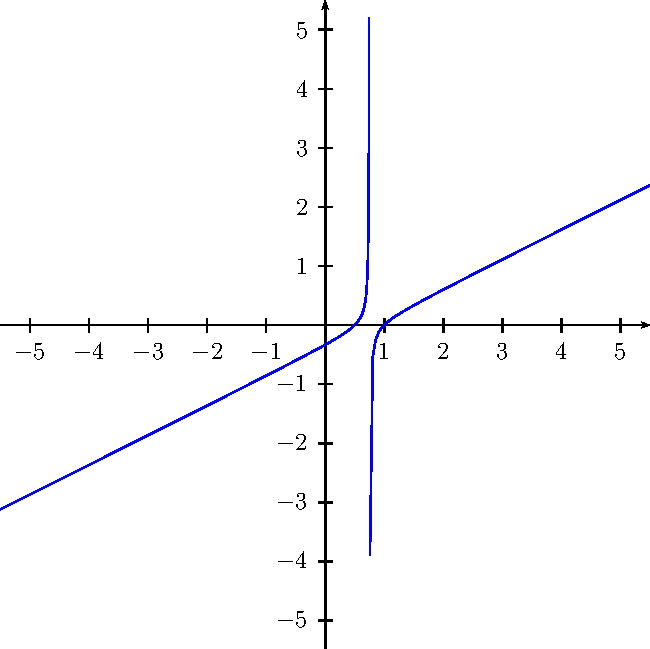
\includegraphics{../images/img005815-3}$$}
    \item \question{$-5x^2+6\sqrt{3}xy+y^2-4 = 0$.}
\reponse{Pour $(x,y)\in\Rr^2$, posons $Q(x,y)= -5x^2+6\sqrt{3}xy+y^2$. Le discriminant de $(\Gamma)$ vaut $-5 -27=-32< 0$.

La conique est du genre hyperbole et de centre $O$. Comme $O\notin(\Gamma)$, $(\Gamma)$ est plus précisément une hyperbole de centre $O$.
Les asymptotes sont fournies par l'égalité $Q(x,y)=0$ et sont donc les droites d'équations $y=(-3\sqrt{3}\pm4\sqrt{2})x$.

La matrice de $Q$ dans la base canonique est $M=\left(
\begin{array}{cc}
-5&3\sqrt{3}\\
3\sqrt{3}&1
\end{array}
\right)$. Son polynôme caractéristique est $\chi_M=X^2+4X-32 = (X-4)(X+8)$. Ensuite, $M = PD{^t}P $ où $P=\frac{1}{2}\left(
\begin{array}{cc}
\sqrt{3}&1\\
-1&\sqrt{3}
\end{array}
\right)$ et $D =\text{diag}(-8,4)$.

Les formules de changement de repère s'écrivent $\left\{
\begin{array}{l}
x=\frac{1}{2}(\sqrt{3}X+Y)\\
y=\frac{1}{2}(-X+\sqrt{3}Y)
\end{array}
\right.$ ou aussi $\left\{
\begin{array}{l}
X=\frac{1}{2}(\sqrt{3}x-y)\\
Y=\frac{1}{2}(x+\sqrt{3}y)
\end{array}
\right.$.

Dans $\mathcal{R}'(O,e_1,e_2)$, $(\Gamma)$ a pour équation $-8X^2+4Y^2-4=0$ ou encore $-\frac{X^2}{(1/\sqrt{2})^2}+Y^2 = 1$. Donc $a=\frac{1}{\sqrt{2}}$, $b=1$ et $c=\sqrt{a^2+b^2}=\sqrt{\frac{3}{2}}$. 

\textbf{Eléments de l'hyperbole dans $\mathcal{R}'$ puis $\mathcal{R}$.} L'axe focal est $(O,e_2)$ c'est-à-dire la droite d'équation $X=0$ dans $\mathcal{R}'$ ou encore $y=\sqrt{3}x$ dans $\mathcal{R}$.

- Les \emph{sommets} sont les points $B$ et $B'$ de coordonées $(1,0)$ et $(-1,0)$ dans $\mathcal{R}'$ et donc de coordonnées $\left(\frac {1}{2},\frac{\sqrt{3}}{2}\right)$ et $\left(-\frac {1}{2},-\frac{\sqrt{3}}{2}\right)$ dans $\mathcal{R}$.

- \emph{Excentricité, foyers, directrices.} $c=\sqrt{\frac{3}{2}}$ puis $e=\frac{c}{b}=\sqrt{\frac{3}{2}}$. Les foyers $F$ et $F'$ ont pour coordonnées $\left(0,\sqrt{\frac{3}{2}}\right)$ et  $\left(0,-\sqrt{\frac{3}{2}}\right)$ dans $\mathcal{R}'$ et donc $\left(\frac{\sqrt{3}}{2\sqrt{2}},\frac{3}{2\sqrt{2}}\right)$ et  $\left(-\frac{\sqrt{3}}{2\sqrt{2}},-\frac{3}{2\sqrt{2}}\right)$ dans $\mathcal{R}$.

En ce qui concerne les directrices, $K=O +\frac{1}{e}\overrightarrow{OB}=\left(0,\sqrt{\frac{2}{3}}\right)_{\mathcal{R}'}$. Les directrices sont les droites d'équations respectives $Y=\sqrt{\frac{2}{3}}$ et $Y=-\sqrt{\frac{2}{3}}$ dans $\mathcal{R}'$ ou encore d'équations respectives $x+\sqrt{3}y=\frac{4}{\sqrt{6}}$ et $x+\sqrt{3}y=-\frac{4}{\sqrt{6}}$.

$$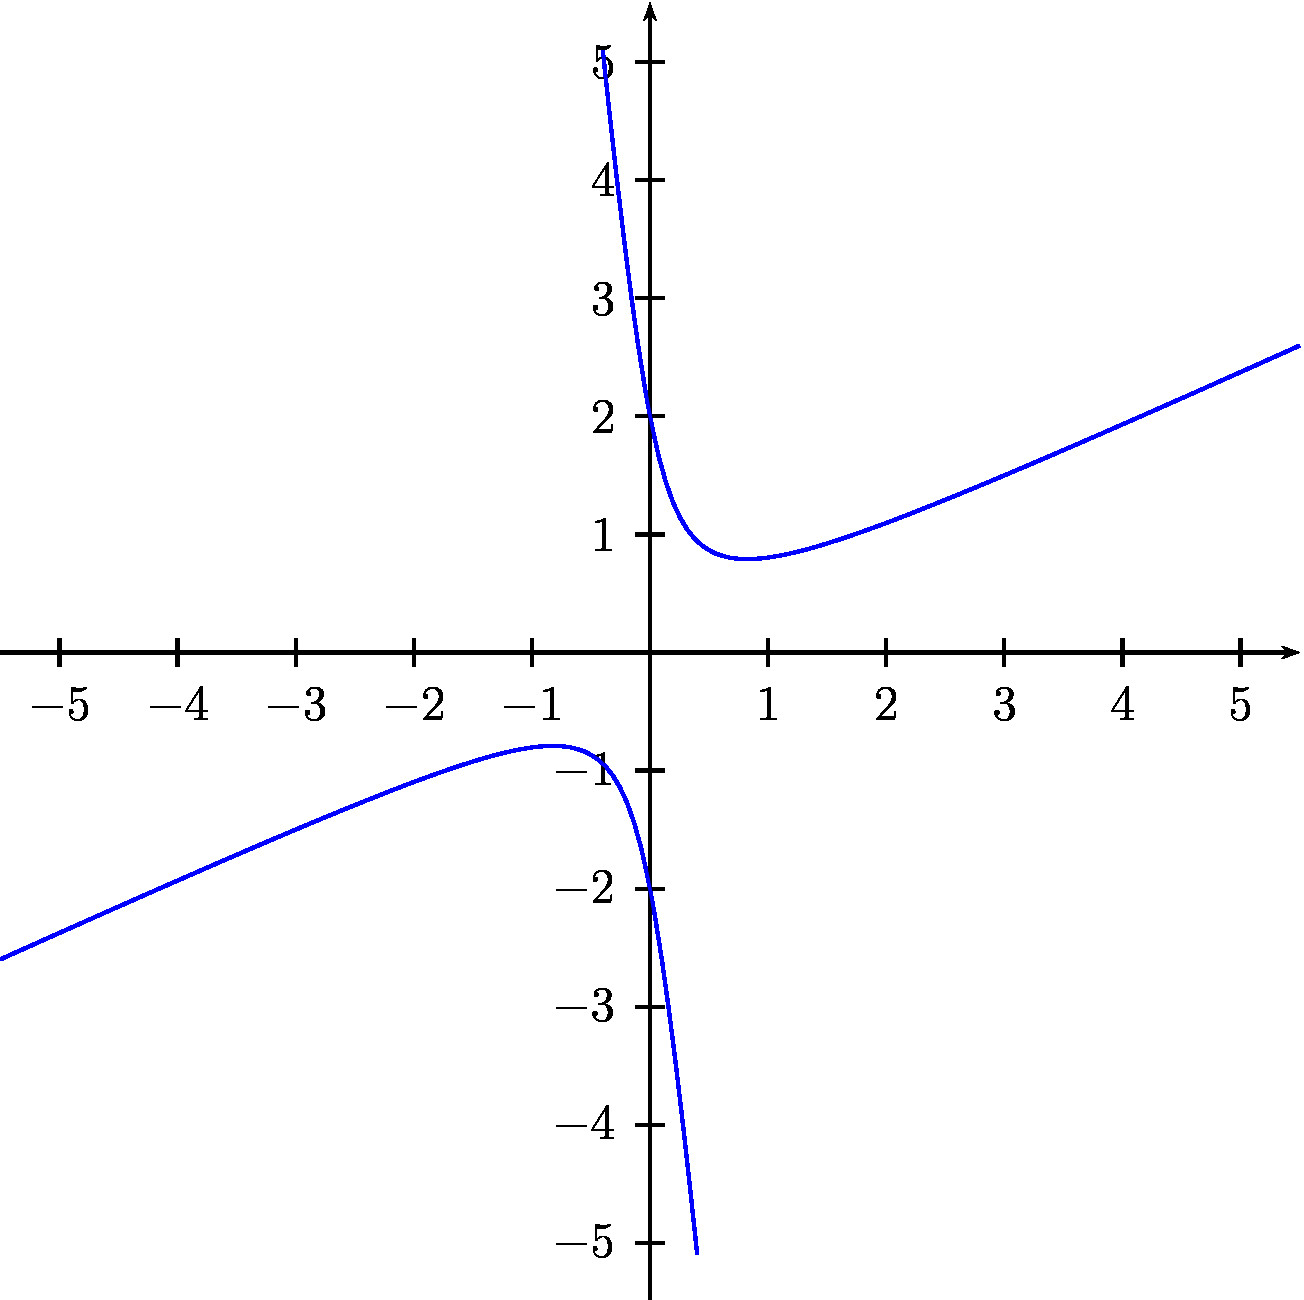
\includegraphics{../images/img005815-4}$$}
    \item \question{$4x^2+12xy+9y^2-2x+1 = 0$.}
\reponse{L'équation proposée s'écrit $(2x+3y)^2- 2x+1 = 0$. Il s'agit d'une conique du genre parabole de direction asymptotique éventuelle $2x+3y = 0$.

Posons $X =\frac{1}{\sqrt{13}}(2x+3y)$ et $Y =\frac{1}{\sqrt{13}}(3x-2y)$ ou encore $x =\frac{1}{\sqrt{13}}(2X+3Y)$ et $y =\frac{1}{\sqrt{13}}(3X-2Y)$.

Dans $\mathcal{R}'=(O,X,Y)$, $(\Gamma)$ admet pour équation cartésienne :

\begin{align*}\ensuremath
13X^2 -\frac{2}{\sqrt{13}}(2X+3Y) + 1= 0&\Leftrightarrow 13\left(X-\frac{2}{13\sqrt{13}}\right)^2 -\frac{6}{\sqrt{13}}Y+\frac{165}{169}= 0\\
 &\Leftrightarrow\left(X-\frac{2}{13\sqrt{13}}\right)^2=\frac{6}{13\sqrt{13}}\left(Y-\frac{55}{26\sqrt{13}}\right)
\end{align*}

Ceci montre que $(\Gamma)$ est une parabole, fournit le paramètre $p =\frac{6}{13\sqrt{13}}$  puis les éléments de $(\Gamma)$ dans le repère $\mathcal{R}'$ : 

$S=\left(\frac{2}{13\sqrt{13}},\frac{55}{26\sqrt{13}}\right)_{\mathcal{R}'}$  puis $F = S +\frac{p}{2}(0,1)_{\mathcal{R}'}=\left(\frac{2}{13\sqrt{13}},\frac{61}{26\sqrt{13}}\right)_{\mathcal{R}'}$ et $K = S -\frac{p}{2}(0,1)_{\mathcal{R}'}=\left(\frac{2}{13\sqrt{13}},\frac{49}{26\sqrt{13}}\right)_{\mathcal{R}'}$  et donc $(D)$ : $Y= \frac{49}{26\sqrt{13}}$.

\textbf{Eléments de $(\Gamma)$ dans le repère $\mathcal{R}$.}

 
$S\left(\frac{173}{338},-\frac{49}{169}\right)_{\mathcal{R}}$  puis $F\left(\frac{191}{338},-\frac{55}{169}\right)_{\mathcal{R}}$   et $(D)$ :  $3x-2y=\frac{49}{26}$.

$$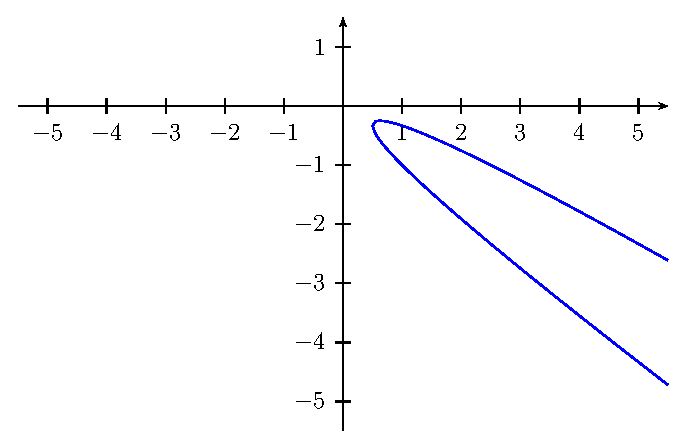
\includegraphics{../images/img005815-5}$$}
    \item \question{$(x-y+1)^2+(x+y-1)^2 = 0$.}
\reponse{$(\Gamma)$ est le point d'intersection des droites d'équations respectives $x-y+1 = 0$ et $x+y-1 = 0$ à savoir le point de coordonnées $(0,1)$.}
    \item \question{$x^2+y^2-3x-y+2=0$.}
\reponse{L'équation s'écrit $\left(x-\frac{3}{2}\right)^2 +\left(y-\frac{1}{2}\right)^2=\frac{1}{2}$. $(\Gamma)$ est le cercle de centre $\left(\frac{3}{2},\frac{1}{2}\right)$ et de rayon $\frac{1}{\sqrt{2}}$.}
    \item \question{$x(x-1)+(y-2)(y-3) = 0$.}
\reponse{On reconnait une équation du cercle de diamètre $[AB]$ où $A(0,2)$ et $B(1,3)$.}
    \item \question{$(x+2y-4)(x-y-1)=3$.}
\reponse{Si on pose $X = x+2y-4$ et $Y = x-y-1$, l'équation s'écrit $XY = 3$ ce qui montre immédiatement que la courbe est une hyperbole dont les asymptotes sont les droites d'équations respectives $x+2y-4= 0$ et $x-y-1=0$ et donc de centre le point d'intersection de ces deux droites $\Omega(2,1)$. Ce changement de repère non orthonormé ne peut pas fournir davantage et si on veut les éléments métriques de l'hyperbole, il faut revenir aux méthodes de 3) ou 4).}
    \item \question{$(2x+y-1)^2-3(x+y) = 0$.}
\reponse{De nouveau, si on pose $X = 2x+y-1$ et $Y = x+y$ (ou même $Y=3(x+y)$) , l'équation s'écrit $X^2 = 3Y$. Le nouveau repère est quelconque mais on peut tout de même affirmer que la courbe est une parabole de direction asymptotique $2x+y=0$.
Avec cette équation, on ne lit cependant aucun des éléments métriques de celle-ci.}
\end{enumerate}
}
